\section{Semantic Modelling} \label{sec:sem_mod}
%These code properties act as contextual information for the vulnerability.

%\todo {\color{blue} Define code property and explain each of the following in details with some examples.}
Due to the dramatic difference in the syntax representations of the binary generated from different compilers, architectures and platforms, \tool leverage on two types of semantic models
%, generated from partial traces, 
to extract semantic features: (1) state-based semantic model and (2) abstract semantic model. As discussed later, each model complement each other on extracting semantic features, which are later fed into the machine learning framework. State-based semantic model gives the low-level perspective of the function (e.g., the effect of a function on the memory, flags and registers), whereas abstract-semantic model gives the high-level understanding of the function (e.g., the high-level operations carried out by the function). In the following sub sections, we'll elaborate on them in detail.
%These complementing features summarize the behavior of the same binary code at different levels to achieve an accurate and yet robust matching cross compilers, architectures and platforms.
%under investigation so that they complement each other and give better understanding of the program.
%On the other hand, syntactic features try to explain the high-level behavioural aspects of the binary code (e.g., type of operation carried out, such as data movement or arithmetic operation).


\subsection{State-based Semantic Modelling} \label{subsec:stat_sem}
State-based semantic model aims to capture the execution effect of the binary code in terms of machine state updates. Lets consider the following simple machine (adapted from \cite{de2015micro}) using which we explain the state transitions during program execution. Later, these state transitions are modelled using state-based semantic models.

%\subsubsection*{Simple Machine} \label{subsubsubsec:bas_mach}
Assume this simple machine has a fixed set of general-purpose registers, condition-code flag registers and a program counter (\textit{pc}) register. Consider the following (subset of) common instructions of the machine:
\begin{equation*}
inst ::= \mathsf{Mov} \: r_s\, r_d\; \vert \; \mathsf{Binop_\otimes} \: r_1\, r_2\, r_d\,f_d \; \vert \; \mathsf{Load} \: r_p\, r_d\; \vert \; \mathsf{Store} \: r_p\, r_s 
\end{equation*}
where $\otimes \in \lbrace \div, \times, \leq, \geq, \ldots\rbrace$. A machine state is characterised by a tuple ($mem, reg, flag, pc$) of a word-addressable memory \textit{mem} (a partial function from words to words), a register file \textit{reg} (a function from register names to words), a condition-code flag file \textit{flag} (a function from flags names to words) and a pc value (a word). In the original formalization, in \cite{de2015micro}, flag is not considered as part of machine state. However, our models are generated from partial traces (discussed in section \ref{subsec:partial_trace}), hence, its is essential to consider the state of condition-code flags (e.g., $CF, PF, \ldots$) in similarity computation, where at a given program point, across two different binary functions, if the state of condition-code flags is identical then it is an indication that those two functions perform similar operations at the machine-code level. It is important to note that the memory is a partial function; trying to address outside of the valid memory (by trying to fetch the next instruction from an invalid address, or loading from or storing to one) halts the machine.

A typical step rule for this machine is written like this:
\\
\begin{equation*}
\begin{aligned}
\mathnormal{\frac{ \splitfrac{mem[pc]=i \quad decode \: i = \; \mathsf{Binop_\otimes} \: r_1\, r_2\, r_d\,f_d \quad reg[r_1]=w_1}{\splitfrac{reg[r_2]=w_2 \quad reg^\prime = reg[r_d \leftarrow w_1 \otimes w_2]}{flag^\prime = flag[f_d \leftarrow w_1 \otimes w_2]\hfill}\hfill \mathsf{(Binop)}}}{(mem, reg, flag, pc) \rightarrow (mem, reg^\prime, flag^\prime, pc+1)}}
\end{aligned}
\end{equation*}
\\
Let's read this rule in detail. Looking up the memory word at address \textit{pc} yields the word \textit{i}, which should correspond to some instruction (i.e., an element of the \textit{inst} set defined above)via  partial function \textit{decode}.  In this case, that instruction is $\mathsf{Binop_\otimes} \: r_1\, r_2\, r_d\, f_d$. Registers $r_1$ and $r_2$ contain the operands $w_1$ and $w_2$, respectively. The notation $reg[r_d \leftarrow w_1 \otimes w_2]$ denotes a partial function that maps $r_d$ to $w_1 \otimes w_2$ and behaves like $reg$ on all other arguments. Similarly, $flag[f_d \leftarrow w_1 \otimes w_2]$ denotes the partial function that maps $f_d$ to the side-effects (if any) of $w_1 \otimes w_2$ on the conditional flags. The next machine state is calculated by updating the register and conditional flag files, incrementing the pc, and leaving the memory unchanged. For example, assume zero-flag is set to 0 ($\mathtt{ZF\;=\;0}$) and the registers $\mathtt{EAX}$ and $\mathtt{EBX}$ holds the values $\mathtt{1}$ and $\mathtt{-1}$, respectively, the execution of an instruction `$\mathtt{ADD\;EAX, EBX}$' (binary operation) leads to following state transition: $\mathtt{EAX}$ now holds the value 0 (i.e., $1\mapsto0$), zero-flag is set to 1 (i.e., $0\mapsto1$) and the program counter is incremented, leaving memory and all other registers and flags unchanged.  

The step rule for $\mathsf{Store}$ instruction can be written as follows: 
\\
\begin{equation*}
\begin{aligned}
\mathnormal{\frac{ \splitfrac{mem[pc]=i \quad decode \: i = \; \mathsf{Store} \: r_p\, r_s \quad reg[r_p]=w_p}{reg[r_s]=w_s \quad mem^\prime = mem[w_p \leftarrow w_s] \hfill}\mathsf{(Store)}}{(mem, reg, flag, pc) \rightarrow (mem^\prime, reg, flag, pc+1)}}
\end{aligned}
\end{equation*}
\\
where it stores the value contained in the register $r_s$ in the memory location pointed to by the register $r_p$. The next state is calculated by updating the memory, incrementing the pc and leaving the register and conditional flag files unchanged. Similarly, we can write the step rule for all other instructions supported by the machine. 
\todo{Should I include the step rules for all instructions supported by REIL IR?}
%\todo{Write a step rule that modifies the }
~\\
\\
The updates made by an instruction on the machine state (as shown by step rules above) are represented by a quantifier-free bit-vector (QFBV) formula.  That is, the function $\langle\!\langle \cdot \rangle\!\rangle$ converts an instruction-sequence into a QFBV formula. The methodology for this conversion can be found elsewhere \cite{lim2011symbolic}. QFBV formula for an instruction sequence is a  2-vocabulary formula that specifies a state transformation 
%(i.e., $\langle$pre-state$\rangle \rightarrow \langle$post-state$\rangle$)
, where the primed vocabulary (e.g., $\textit{mem}^\prime$) is the post-state vocabulary, and the unprimed vocabulary (e.g., \textit{mem}) is the pre-state vocabulary. It is important to note that in QFBV formulas the state transition of the program counter \textit{pc} (i.e., $pc^\prime = pc+1$) is omitted as it doesn't not contribute to compare two different programs. Hence, in \tool, the machine state is essentially characterised by a triple (\textit{mem, reg, flag}).
\note{We generate QFBV formulas for the entire partial trace, hence, state of \textit{pc} plays an insignificant role in semantic matching.}

The QFBV formulas for a few IA-32 instructions are given in figure \ref{fig:example-qfbv}. The first instruction loads the value in the memory location pointed to by the base-pointer (i.e.,  $\mathtt{EBP}$) to the  $\mathtt{EAX}$ register. The second instruction pushes the 32-bit constant value 0 on the stack and the third instruction loads  $\mathtt{EAX}$ with the value  $\mathtt{EBP+4}$ (without modifying the value of any flag).


\begin{figure}[!h]
\begin{center}\vspace{-1mm}
%\scriptsize
\begin{itemize}
  \item[] $\mathtt{\langle\!\langle mov \;\; eax, [ebp]\rangle\!\rangle\equiv EAX^\prime = Mem(EBP)}$
  \item[] $\mathtt{\langle\!\langle push \;\; 0\rangle\!\rangle\equiv ESP^\prime=ESP-4 \wedge Mem^\prime = Mem[ESP-4\mapsto 0]}$
  \item[] $\mathtt{\langle\!\langle lea \;\; eax, [ebp+4]\rangle\!\rangle\equiv EAX^\prime = EBP + 4}$
\end{itemize}
~\\
\caption{QFBV formulas for example IA-32 instructions}
\label{fig:example-qfbv}
\end{center}
\end{figure}
Functions, in a real-world program, can easily have several thousand instructions and hence, it is not practical, in terms of scalability, to compare each instruction in the signature function with the target function. In addition, comparison of single instructions will result in high false positive rate, where an instruction can be too common and too small to capture the underlying function semantics.  For example, the instruction \texttt{mov eax, [ebp]}, in its own, does not tell anything about the function and can appear in functions that are totally dissimilar.  Therefore, in \tool, we capture the effect of each partial trace (not single instructions) has on the machine state 
%register, flag and memory locations written to or updated 
during execution.
\note{It is important to note that partial traces, in general, have lots of inputs (i.e., registers, flags and memory locations read from, called \textit{input arguments}) and outputs (i.e., registers, flags and memory locations written to, called \textit{output arguments}). Hence, from extracted QFBV formulas, the input and output arguments are identified and they are 
%organized in such a way that output arguments are expressed by input arguments}.
represented in the form: $\langle$output argument$\rangle$ $=\langle$input argument(s)$\rangle$. The relationship between input and output arguments are called \textit{symbolic expressions}.}
%That is, using QFBV formulas, we capture the machine-state transitions over each partial trace, resulting in a \texttt{set} of $\langle$pre-state, post-state$\rangle$ pairs for each function under investigation.  

%That is, we accumulate the QFBV formulas over a partial trace and derive an expression (called, symbolic expression or S-Expression) for each register, flag and memory locations written to during the execution.  

%the QFBV formulas are accumulated over a rage of basic-blocks (in our case, partial traces) and from the accumulated QFBV formulas, the effect of

%That is, from each partial trace, QFBV formulas are collected and using them the effect of   
 
%A program state is characterised by register, control flag and memory values.
%Formally, we define a program state as a triple $$(RegMap, FlagMap, MemMap)$$
%where $RegMap$, $FlagMap$, and $MemMap$ map each register, control flag, and memory location to a value, respectively.
%The effect of a binary code on the program states, is represented by a set of symbolic formulae, called \textit{symbolic expressions}.
%
%%\begin{mydef}
%%\emph{(\textbf{Symbolic Expression}) } Symbolic formulae that represent the effects of executing a piece of code, on the program-state, in-terms of system registers, control flags and memory values.
%%\end{mydef}
%\begin{eqnarray}
%\label{eq:sym_exp}
% \text{\texttt{push ebp}} &\equiv& \text{(\texttt{(ESP' = ESP-4})} ~\wedge \nonumber \\
%   &&  \text{(\texttt{[ESP-4] = EBP})}~
%\end{eqnarray}
%For example, the symbolic sexpression of an instruction `\texttt{push ebp}' is shown in Equation \ref{eq:sym_exp} (assuming in an IA-32 machine). It can be seen that when \texttt{EBP} register is pushed into the stack, the value of \texttt{ESP} register changes to \texttt{ESP-4} and the memory location \texttt{[ESP-4]} is now holding the value of \texttt{EBP} register. Here, prime (\texttt{'}) indicates the post execution state. In contrast to other symbolic expression\footnote{Symbolic expression and semantic features are used interchangeably in this paper.} based program representation techniques~\cite{pewnycross,lakhotia2013fast,ruttenberg2014identifying}, we extract semantic features at various granularity levels (i.e., beyond basic-block levels) to measure the effect of partial traces at different program points. Partial trace models are explained in details later under function model generation module.

%\note{discuss the memory reads and writes briefly}

\subsection{Abstract Semantic Modelling} \label{subsec:abs_sem_mod}

The limitation in state-based semantic model is that it lacks some of the details, readily available from the machine code, that can be leveraged on to understand the intentions (or objectives) of the partial traces. That is, state-based models are too low-level as such they are incapable of capturing the high-level behavioural characteristic of partial traces (discussed in section \ref{subsec:partial_trace}). In addition, the effects of library calls are not interpreted in state-based models. That is, the instructions \texttt{call CreateFile} and \texttt{call GetTime} are treated in the same way, whereas, in reality, the effects of these two library calls are totally different. Hence, in \tool, we compensate the limitations of state-based semantic models using abstract semantic models, where we capture the high-level behavioural characteristics, of each partial trace, using \textit{abstract semantic} graphs. The major challenge in extracting the behavioural characteristics from machine-code is that the assembly instructions (i.e., syntax) and the API (Application Programming Interface) names are not consistent across architectures (ARM Vs. x86) and platforms (Linux Vs. Windows), hence, they need to be unified.\todo{Here, I need to explain, in detail, why IR is not used to extract high-level characteristics. The main reason is, IR is too low-level, where a simple `$\mathtt{pushfd}$' instruction in x86 takes around 40 REIL instructions to implement, hence, not suitable to extract high-level behavioural characteristics.}

\subsubsection{Unified Abstraction} 
The assembly instructions extracted from  machine code can be directly used to represent the high-level behavioural characteristics. For example, $\mathtt{MOV\;EAX,EBX}$ tells that the value in source register $\mathtt{EBX}$ copied to the destination register $\mathtt{EAX}$. Similarly, the instruction $\mathtt{call\;CreateFile}$ indicates that a new file is created (or an existing file is opened). However, this representation shamelessly fail in the event of cross-architecture and -platform experiments due to the differences in instruction set architectures and the difference in API names, supported by different platforms. Therefore, to overcome these limitation, in abstract semantic models, the high-level behaviours are characterised by unified abstraction of operations (called, \textit{operation type}) and API invocations (called, \textit{API type}). That is, we abstract the operations carried out by the low-level instructions and the APIs invoked during the execution, such that they are architecture and platform agnostic (hence the name, \textit{unified abstraction}). 
%the high-level intentions are characterised by two behavioural abstractions: (1) \textit{operation type}, and (2) \textit{library call type}. That is, instead of using instructions and library calls directly to represent the high-level intentions, we leverage on their abstractions.

\begin{table}[t]
\caption{Categorization of assembly instructions based on their high-level operations. \textsuperscript{$\spadesuit$}A common trick to move 0 to a register is by \texttt{xor}ing the register with itself, similarly, \texttt{lea} can be used to perform arithmatic operations}\label{tab:opt-cat}
\begin{center}
{\scriptsize
\begin{tabular}{|c|c|}
  \hline
  \textbf{Operation type} & \textbf{Sample instructions} \\
  \hline
  Data movement & \texttt{mov, movsx, xchg, xor\textsuperscript{$\spadesuit$}}\\
  \hline
  Arithmetic  & \texttt{add,adc,sub,sbb, lea\textsuperscript{$\spadesuit$}} \\
  \hline
  Logic & \texttt{and,or,not,xor}\\
  \hline
  Shift-rotate & \texttt{shr,shl,sal,rcl,rcr}\\
  \hline
  String  & \texttt{cmps,cmpsb,cmpsw,cmpsd} \\
  \hline
  %Loop & \texttt{loop,loopne,loopnz,loope}\\
  %\hline
  %Control transfer & \texttt{jno,jnp,jns,jo,jp,jpe}\\
  %\hline
  Stack  & \texttt{pusha, pushf, popa, popf} \\
  \hline
  Conversion & \texttt{cbw, cwd, cwde, cdq, csq}\\
  \hline
  %I/O  & \texttt{in, out} \\
  %\hline
 %Floating-point & \texttt{fld, fstp}\\
  %\hline
 % Halt & \texttt{hlt}\\
 % \hline
 Flag  & \texttt{cld,clc,stc,std,sti} \\
  \hline
  \end{tabular}
}
\end{center}
\end{table}

\begin{table}[t]
\caption{Abstraction of API calls based on the task accomplished}\label{tab:lib-cat}
\begin{center}
{\scriptsize
\begin{tabular}{|c|c|}
  \hline
  \textbf{API type} & \textbf{Sample API calls} \\
  \hline
  String & \texttt{strcpy, strcat}\\
  \hline
  Memory  & \texttt{memcpy, memset} \\
  \hline
  Network & \texttt{socket, gethostbyname }\\
  \hline
   File & \texttt{CreateFile, fopen}\\
  \hline
  Process  & \texttt{CreateProcess, pthread\_exit} \\
  \hline
 Crypto & \texttt{crypt, encrypt}\\
  \hline
  Synchronization  & \texttt{CreateMutex, pthread\_mutex\_init} \\
  \hline
  Heap & \texttt{brk, HeapAlloc}\\
  \hline
  \end{tabular}
}
\end{center}
\end{table}

%In addition to low level semantic features, \tool leverages on high-level semantic features extracted from the functions to understand the operations carried out by the binary code. Combining state-based semantic and abstract semantic features gives the good mix of functions properties that can be effectively used to search similar functions from the target function pool. To this end, we are considering two behavioural abstractions: (1) operation type, and (2) library call invocations.

\begin{itemize}

\item \textbf{Operation type}: Here, we look into the actual machine code to infer the possible operations, at a given abstraction level, that a partial trace can perform. To this end, we have identified several types of operations that are architecture agnostic. That is, these operation types are uniform across different architectures. They are as follows: data movement, arithmetic operation, logic operation, shift and rotate operation, string operation, 
%loop operation, control transfer operation, 
stack operation, conversion (or sign extension) operation, 
%I/O operation, 
%floating-point operation 
%halt operation 
and flag manipulation. Table \ref{tab:opt-cat} list the operation types used in \tool.

\item \textbf{API type}: API invocations give a valuable hint about the activities that are likely to be carried by the partial trace. For example, the presence of \texttt{strcpy} function from \texttt{libc} library indicates that the partial trace is likely to handle strings. We can directly include the API name as part of the feature, if both the search query and the target functions are compiled for the same platform (e.g., Linux) and uses identical API calls. However, in real-world, this assumption is too restrictive, even within the same platform, as there are several alternate APIs available to accomplish a given task  (e.g., in Windows, to create a file, a programmer can either use \texttt{CreateFile} API call or \texttt{OpenFile} API call with open switch).  Thus, in abstract semantic models, to account for the differences in API calls that accomplish similar task and to enable cross-platform (e.g., Windows vs. Linux) analysis, we map API invocations to their corresponding types. For example, string functions such as \texttt{strlen} and \texttt{srtncat} are mapped to \textit{string} API type. That is, \texttt{strlen} and \texttt{srtncat} APIs are, in general, used to manipulate a given string, hence, abstracted to `string' API type. Table \ref{tab:lib-cat} lists the API types used in \tool.
\end{itemize}

\subsubsection{Abstract Semantic Graph} 
The high-level behavioural characteristics extracted from partial traces alone is not very useful unless it is represented systematically to capture the complete picture. For example, consider the following instruction sequence and the corresponding abstractions.

\begin{itemize}
\itemsep0em 
  \item[] $\mathtt{mov \;\; eax, [ebp] \quad\quad// data\_movement\_from\_memory}$
  \item[] $\mathtt{push \;\; eax \quad\quad// stack\_operation\_store}$
  \item[] $\mathtt{call \;\; socket \quad\quad// network\_connection}$
\end{itemize}
 
It can be seen that abstract information extracted from each instruction alone, without any systematic representation, doesn't fully express the underlying intention of this code segment. One major limitation in representing the high-level behavioural characteristics  as a set (e.g., 
%$\mathtt{data\_movement\_from\_memory,}$  $\mathtt{stack\_operation\_store,}$  $\mathtt{network\_connection}$
\{\textit{data\_movement\_from\_memory, stack\_operation\_store, network\_connection}\}) is that the relationship between behaviour is completely ignored, where in the above code segment, all three instructions are related (i.e., data dependent). Hence, its vital to reflect the relationship between extracted behavioural characteristics. To this end, we use directed graph to represent the high-level behaviour and their relationship, where it is referred to as \textit{abstract semantic graph} and the definition is given below.

\begin{mydef}
\emph{(\textbf{Abstract Semantic Graph}) }  Abstract Semantic Graph is a directed acyclic graph, where the nodes represent the high-level behaviour and the edges represent the relationship between two high-level behaviours. Here, relationship refers to the data dependence between two behavioural characteristics.
\end{mydef}

It is important to note that identifying the data-dependence relationship between two high-level behaviours is not feasible as the extracted behaviours are too abstract. Hence, to build the abstract semantic graph, we leverage on the data-dependence between assembly instructions and propagate the relationship to the behaviour level. This is from the notion that if two assembly instructions are data-dependent, their high-level abstractions (i.e., behaviour) are too data-dependent. To this end, we rely on the \textit{def-use} chains to identify the data-dependence between assembly instructions. The abstract semantic graph for the above code segment will look like this: 

\begin{figure}[!h]
\begin{center}\vspace{-1mm}
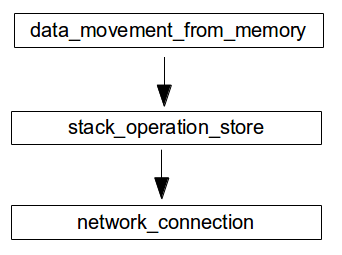
\includegraphics[height=4cm, width=6cm]{srj-figures/srj-graph.png} \vspace{-1mm}
\caption{Abstract semantic graph}
\label{fig:abs} %\vspace{-1mm}
\end{center}
\end{figure}

\begin{MyAlgo}[!ht]{-4.9cm} %increase or decrease margin, span across columns
 \DontPrintSemicolon
 \KwData{partial trace $\wp$}
 \KwResult{set of abstract semantic graphs $G$}
% \SetKwFunction{algo}{ExtractTracelets}\SetKwFunction{proc}{Extract}
% \SetKwProg{myalg}{Algorithm}{}{}
% \myalg{\algo{$CFG$}}{
  $G \longleftarrow \emptyset$ \;%\tcp*{set of abstract semantic graphs}
 \ForEach{{\upshape instruction} i {\upshape in} $\wp$}{
  %\tcc{write the algo here}
  %$kT \longleftarrow kT \cup Extract(b, k)$\;
  $D_i \longleftarrow  \mathtt{getDef}(i)$\;
  $g \longleftarrow \emptyset$\;
  $j := i.\mathtt{Next}$\tcp*{$j$ is the next instruction after $i$ in $\wp$}
   \ForEach{{\upshape instruction} j {\upshape in} $\wp$}{
   $U_j \longleftarrow  \mathtt{getUse}(j)$\;
   $D_j \longleftarrow  \mathtt{getDef}(j)$\;
   \If{$U_j \in D_i $}{
	   	$g := g \cup {v_i \rightarrow v_j}$\; 
   		 \If{$\mathtt{getType}(j) == \mathtt{DATA\_MOVEMENT}$}{
   			$D_i := D_i \cup D_j$\;
   		}
     }
      \If{$D_j \in D_i $}{
	   	$D_i := D_i \setminus D_j$\;
   		}
   		\If{$D_i ==  \emptyset $}{
   			%\If{$g$ {\upshape not in}  $G$}{
   			\If{$\mathtt{isPresent}(g,G) = 0$}{
   		 		$G := G \cup g$\; 
   		 	}
	   	   $break$\;
   		}
   }
  }
  \Return ${G}$
  %}
  %\setcounter{AlgoLine}{0}
  %\SetKwProg{myproc}{Procedure}{}{}
  %\myproc{\proc{b, k}}{
  %\eIf{$k == 1$}{
   % \Return $b_s$
  %}{
   %\Return $\bigcup b \times Extract(b^\prime, k-1)$\;
  %}
  %}
  \\
 \caption{Abstract semantic graph constraction using def-use chain}\label{algo:def-use}
\end{MyAlgo}

From figure \ref{fig:abs}, it can be seen that the relationship between high-level behaviours gives the complete picture of what the code segment is doing. That is, from the above abstract semantic graph, we can infer that some data from the memory is sent over the network.  Algorithm \ref{algo:def-use} presents the def-chain algorithm that is used to identify the data dependence between assembly instructions. Here, we define several functions to accomplish our tasks. They are; (1) $\mathtt{getDef(i)}$ returns the variables defined in instruction $i$ (e.g., in `$\mathtt{mov\;eax,ebx}$', the register $\mathtt{eax}$ is defined), (2) $\mathtt{getUse(i)}$ returns the variables used in instruction $i$ (e.g., in the previous instruction, the register $\mathtt{ebx}$ is used), (3) $\mathtt{isPresent(g,G)}$ check whether the abstract semantic graph $g$ is already present in $G$, and (4) $\mathtt{getType(i)}$  returns the type of the instruction $i$. At high-level, for each instruction present in the partial trace, we get the defined variables and iterate through the rest of the instructions to check whether those defined variables are used elsewhere, if found, data dependency between those two instructions are established. Each iteration terminates either (1) reached end of partial trace, or (2) variable defined by instruction $i$ is redefined by another instruction $j$, where $location(i) < location(j)$.
%Thought these code properties helps to identify potential candidate functions in the target program, there are several drawbacks that we need to be aware of. First, it is important to note that some programs may implement their own version of some the library functions, in which case, we may fail to detect the vulnerabilities in functions (if present) that invoke their own version of library function. Fortunately, most of programs still use the standard library functions and thus, we decided to include them as part of the pre-filtering properties. Next, structural information, cannot always be trusted as, in practise, compilers can inline/outline functions and hence, this metric will provide some misleading information. Similarly, operation type may too provide some false indication as some tasks can be achieved with semantically equivalent instruction that belongs two different types in our categorization.

%However, considering the number of functions present in the real world applications, it is very beneficial, in terms of scalability, to have a pre-filtering process in place to select candidate target functions that are likely to contain vulnerability.   Hence, to reduce the negative impact of our properties, we apply weights to each property based on their contribution in pre-filtering. Through evaluation, we identified that library call invocation and operation type properties considerably contributes towards correctly identifying candidate target functions followed by structural property. Therefore, the total synthetic similarity ($sim_{tot}$) is measured as follows:
%\begin{equation}
%sim_{tot} = w_l*sim_l + w_o*sim_o + w_s*sim_s \label{eq:tot_syn_sim}
%\end{equation}
%where, $sim_l$, $sim_o$ and $sim_s$ refers to similarities based library call invocation, operation type and structural properties, and $w_l$, $w_o$ and $w_s$ refers to their corresponding weights, respectively.